\documentclass[12pt]{beamer}
\usetheme{Warsaw}
\usepackage[utf8]{inputenc}
\usepackage{amsmath}
\usepackage{amsfonts}
\usepackage{amssymb}
\usepackage{graphicx}
\usepackage[font=Times,timeinterval=1,timeduration=2.0,timedeath=0,fillcolorwarningsecond=white!60!yellow,timewarningfirst=50,timewarningsecond=80,resetatpages=2]{tdclock}
\usepackage{tabularx}
\usepackage{array}
\usepackage{multicol}
\usepackage{longtable}
\usepackage{xcolor}
\usepackage{textcomp, gensymb}
\usepackage{pgfplots}
\usepackage[makeroom]{cancel}

\graphicspath{ {./references/} }
\pgfplotsset{
	soldot/.style={color=black,only marks,mark=*},
	holdot/.style={color=black,fill=white,only marks,mark=*},
	compat=1.12
}
\newcolumntype{Y}{>{\centering\arraybackslash}X}
\makeatletter
\def\@listii{\leftmargin\leftmarginii
			  \topsep    2ex
			  \parsep    0\p@   \@plus\p@
			  \itemsep   \parsep}
\makeatother

\begin{document}
\begin{frame}
	\frametitle{Bellwork 9/29}
	\initclock

	\Large
	\[f(x) = \frac{1}{x}\]
	\begin{enumerate}\itemsep2ex
		\item Find $f'(x)$.
		\item Find an equation for the line tangent to $f$ at $x=-2$.
	\end{enumerate}
	\vfill
	\vfill

	\small
	\crono
	\resetcrono{\beamerbutton{reset}}
\end{frame}
\begin{frame}
	\frametitle{Bellwork 9/29 - Solutions, Part 1}

	\large
	\[f'(x) = \displaystyle\lim_{h\to 0}\left(\frac{\frac{1}{x+h}-\frac{1}{x}}{h}\right)\]
	\[=\displaystyle\lim_{h\to 0}\left(\frac{\frac{x-x-h}{x^2+hx}}{h}\right)\]
	\[=\displaystyle\lim_{h\to 0}\left[\frac{-\cancel{h}}{\cancel{h}(x^2+hx)}\right]=\boxed{-\frac{1}{x^2}}\]
\end{frame}
\begin{frame}
	\frametitle{Bellwork 9/29 - Solutions, Part 2}

	\large
	\vfill
	\vfill
	\vfill
	\vfill
	\[y-y_1=m(x-x_1)\]
	\vfill
	\[\implies y-f(-2)=f'(-2)(x+2)\]
	\[\implies y=-\frac{1}{4}(x+2)-\frac{1}{2}\]
	\[\implies \boxed{y=-\frac{1}{4}x-1}\]
	\vfill
	\vfill
	\vfill
	\vfill
\end{frame}
\begin{frame}
	\frametitle{Exercise 1}

	\begin{center}
		\vfill
		Function $f$ is graphed below:
		\vfill
		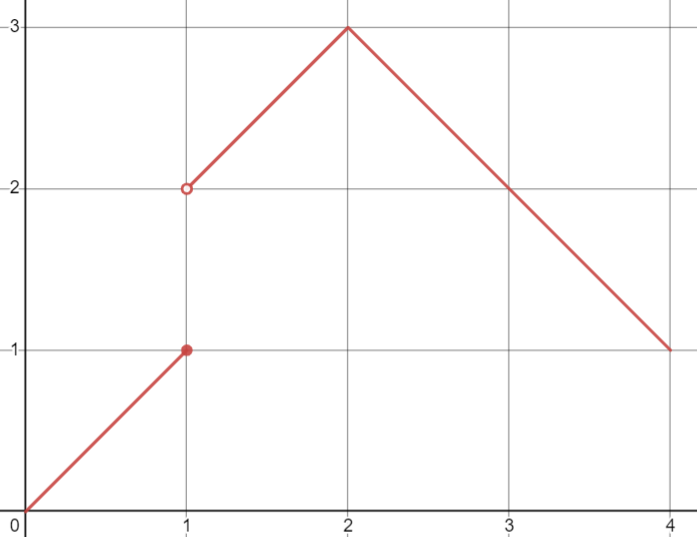
\includegraphics[scale=0.5]{exercise_1_graph.png}
		\vfill
		Sketch $f'(x)$ and find where $f$ is not differentiable.
		\vfill
	\end{center}
\end{frame}
\begin{frame}
	\frametitle{Exercise 1 - Solution}

	\begin{center}
		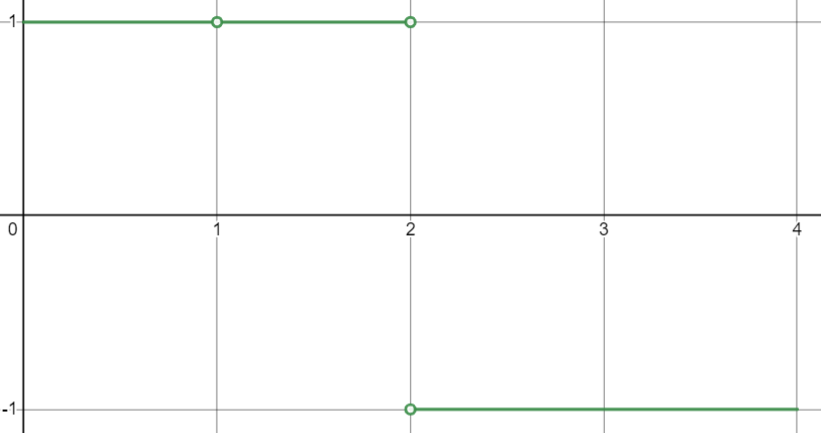
\includegraphics[scale=0.6]{exercise_1_solution_graph.png}
		\vfill
		$\boxed{x=1\text{, }2}$
	\end{center}
\end{frame}
\end{document}